\section{Introduction}

%motivation
The physical laws of motion say that an accelerating car consumes more fuel than a car driving at a constant velocity. %TODO: Citation
If one wants to safe fuel, one should therefore try to accelerate as little as possible. 
However, several factors in todays traffic hinders drivers in driving at a constant velocity. 
These are for example interlacing roads, blocking vehicles, traffic incidents and of cause traffic lights. 
It is esimated at 1.8 bilion danish kroner is lost on fuel each year on vehicles stopping for red lights in traffic lights in Denmark \cite{Vejdir}.

%the problem of traffic lights
Traffic lights hinders the flow of traffic as it blocks vehicles arriving from one direction in order to allow other vehicles to drive through the intersection.
Each direction of the intersection is given a time period in which vehicles are allowed to pass through the intersection. 
From a drivers perspective it is only posible to guess when the light is going to change based on what he has seen so far. 

Locking at Figure \ref{fig:Introduction:network} vehicle $h_2$ is approacing the intersection.
%If he have spottet a red light for some time, it is likly that the signals are going to change soon. He can either, take the chance and keep driving at the same speed, until the last momment where he need to brake. Or he can slow down and limp toward the intersection and then maybe avoid a full stop at the traffic light. 
Now assume that vehicle $h_2$ knows the distance $d_2$ where he have to stop for traffic light $l_1$. Then also assume that vehicle $h_2$ know that in $4$ seconds the traficligh $l_1$ will change to green. Now it is posible to calculate a speed for vehicle $h_2$ such that it drive the distance $d_2$ in $4$ seconds. Then by the time it reach the intersection the signal will have changed and thereby avoiding a full stop.

%problem of not knowing how many other cars are wating in line
The system proposed in this article is designed on the basis that not every vehicle will be using it. 
Because of this, we cannot rely on communication between vehicles and therefore we do not know how many vehicles will be waiting in line for a green light. %TODO this depents on access to induction loop data
Hence we cannot predict the precise distance to the position at a traffic light where the driver must stop due to blocking cars. In Figure \ref{fig:Introduction:network} this can be observed as vehicle $h_1$ drives towards traffic light $l_2$. He believes that the distance to were he have to stop is the distance of $d_1$ however the two blue cars already wating in line, block's a part of the road.

Some traffic lights do not always show the same signal to vehicles going in diffrent directions where it be straight, left or right turn. We model this by having \textit{connections} in the intersection. Each lane have an uniqe identifier as shown in Figure \ref{fig:Introduction:network}. Each posible legal pass throug the intersection is then added to the \textit{connection table} as show in Table \ref{tab:Introduction:connectionTable}.

%Modern traffic lights have sensors known as \textit{induction loops} that can detect vehicles driving on the roads.
%These sensors are used to regulate the signals in relation to the number of vehicles approaching the intersection \cite{Vejdir}. %TODO do we need this?
%If it is possible to reduce the stop-and-go behaviour at traffic lights, it might be possible to reduce the fuel consumption.
%section describing terms of traffic traffic light phase, cycle time ect


%model discribing what we do

\begin{figure}[htb]
\centering
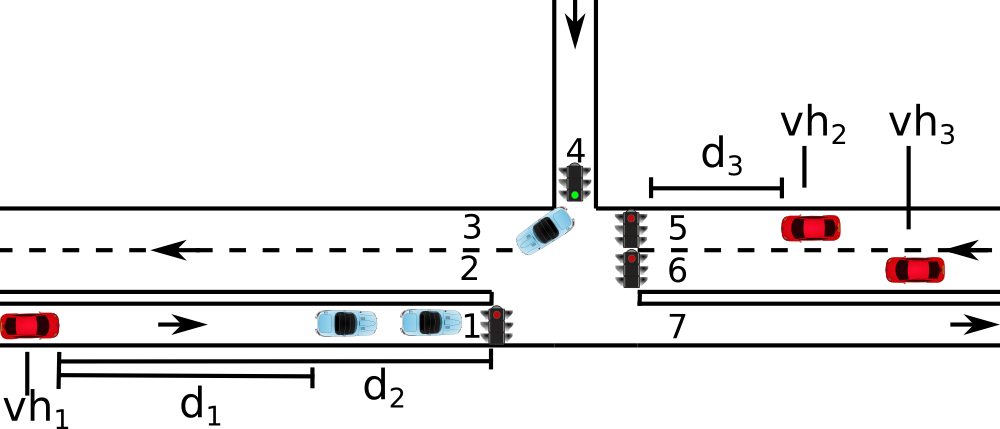
\includegraphics[width=0.5\textwidth]{images/introNetwork.png}
\caption{Eksample network}
\label{fig:Introduction:network}
\end{figure}

\begin{table}[h]
\centering
\begin{tabular}{|l|l|}
\hline
from & to \\ \hline
1 & 7 \\ \hline
4 & 3 \\ \hline
4 & 7 \\ \hline
5 & 3 \\ \hline
6 & 2 \\ \hline
\end{tabular}
\caption{Connection table of the network shown in Figure \ref{fig:Introduction:network} }
\label{tab:Introduction:connectionTable}
\end{table}


%section describing problem with sensors \TODO do we need this?
%A traffic light using only a timer to regulate the traffic is relatively easy to predict if the phases and cycle time is known. 
%However, when we introduce induction loops that are are effected by vehicles ariving in an unpredicteble pattern, then the traffic light will also to some extent become unpredicteble. 

%describe why we do simulation 
The focus of this article is to investigate whether it is possible to reduce fuel consumption at traffic ligths by matching the speed to the traffic lights. We investigate this through simulations with real world map data, traffic data and traffic light programs, both with crossing traffic and road-side senors. %TODO check we do this
%To investigate the extent of this problem we create simulations based on real world map data, traffic data and traffic light programs. 
We use the traffic simulator SUMO (Simulation of Urban Mobility)\cite{sumo} interfaced via TraCI (Traffic Control Interface)\cite{traci} which is a full scall microscopic traffic simulator.

%TODO: outline of the article
//Outline of the article





